\documentclass[10pt]{article}

\usepackage{amsmath}
\usepackage{amssymb}
\usepackage{graphicx}
%\usepackage{picins}
\usepackage{amsthm}
\usepackage{bbm}

\setlength{\voffset}{-28.4mm}
\setlength{\hoffset}{-1in}
\setlength{\topmargin}{20mm}
\setlength{\oddsidemargin}{25mm}
\setlength{\evensidemargin}{25mm}
\setlength{\textwidth}{160mm}
\usepackage{subfigure}

\setlength{\parindent}{0pt}

\setlength{\textheight}{235mm}
%\setlength{\footskip}{20mm}
\setlength{\headsep}{50pt}
\setlength{\headheight}{0pt}

% Paket zur Verwendung einer verbesserten Schriftart
\usepackage{lmodern}

%Language package französisch
\usepackage[english]{babel}
\usepackage[T1]{fontenc}
\usepackage[utf8]{inputenc}


%Hyperref
\usepackage[backref = true]{hyperref}

%Einbinden von Graphen
\usepackage{tikz}

\begin{document}
	
\begin{titlepage}
	\begin{center}
	
		{\Large
			Université de Pierre et Marie Curie 
		}
		\normalsize
		
		Course Project\\[15mm]
		
		{\Huge
			Recherche rapide d’un triangle contenant un point dans un maillage
		}
		\vspace{2cm}
		
		\normalsize
		
		Arne Heimendahl, Olivia Kaufmann
		
		\begin{figure}[t]
			
\includegraphics[scale=0.1]{UPMC_Sorbonne_Universites.png}
		\end{figure}
		
	\end{center}
	\vspace*{75mm}
	
	Supervisor: 
	\medskip
	
	Advisor: 
	\medskip
	
	Submission Date: 13.01.2018 
	
\end{titlepage}

\newpage
\tableofcontents
\newpage

%\pagenumbering{arabic}
%\pagestyle{headings}
	
%\title{Recherche rapide d’un triangle contenant un point dans un maillage}

Adj vis Map, Exp Gnu

O Prom, Adj vis List, find Sommets und Rec

\section{Project description and aim}

The aim of this project is to implement an algorithm which searches for a triangle in a convexe mesh covering a point $(x,y)$. A linear complexity (in number of vertices of the mesh) is desired.

\section{The template class T3 and the class Triangle}

\subsection{The template class T3} \label{T3}

Objects of the class $T3$ represent elements of a three dimensional space in $T$. Hereby, the data type $T$ is defined using a template. Within this project, either $T3<int>$ for the definition of a triangle (see \ref{triangle}) or $T3<double>$ for the definition of the coordinates of a vertex (see X) is used. The private members $x,y$ and $z$ of type $T$ store the entries of the $T3$ vector. The class has a default constructor, a constructor by copy and a constructor creating a vector given the three vector entries. Moreover, the class has operators to access and modify the entries, add to elements of $T3$, multiply an element of $T3$ by a scalar of the type T and calculate the scalar product of two $T3$ vectors. The operator $<$ compares two elements of $T3$, $v_1 = \begin{pmatrix} x_1 & y_1 & z_1 \end{pmatrix}^T$ and $v_2 = \begin{pmatrix} x_2 & y_2 & z_2 \end{pmatrix}^T$, in the following way:
$$ v_1 < v_2 \quad \Leftrightarrow \quad \begin{cases}
 x_1 < x_2 \text{ or }\\
 x_1 = x_2 \text{ and } y_1 < y_2 \text{ or }\\
 x_1 = x_2 \text{ and } y_1 = y_2 \text{ and } z_1 < z_2
\end{cases}. $$ 
This allows a lexicographic ordering of a list of $T3$ elements (see \ref{list}, $T3<int>$). For three $T3$ vectors, which define the vertices of a triangle, the method $ oriented\_vol $ computes the corresponding signed volume. Let $a,b$ and $c$ denote $T3$ vectors. The oriented volume $A_{abc}$ is defined as
$$ A_{abc} = \left( \overrightarrow{ab} \times \overrightarrow{bc} \right)^T \begin{pmatrix} 0 \\ 0 \\ 1 \end{pmatrix} = (b_1-a_1)(c_2-b_2) - (b_2-a_2)(c_1-b_1)$$

The sign is positive for triangles oriented in trigonometric sense. This method is used in the method $promenade$ \ref{promenade} to determine a suitable 'walking' direction.


\subsection{The class Triangle} \label{triangle}
The class Triangle inherits form the class T3. Its derived members $ i,j,k $ are specialized as integers representing the position of its defining vertices in the array of the points of the given mesh. This array is a member of the class mesh in \ref{mesh}. In addition, it has three extra integer members {\itshape neighbor1, neighbor2, neighbor3} representing the position of the adjacent triangles in the array of triangles which is also a member of the class mesh. Notice that theses index lies between zero and the number of triangles minus one. \\
 An adjacent triangle $ t^{'} $ is said to be  {\itshape neighbor1 } of a triangle $ t $ if, saying $ i $ represents the first index of a vertex of $t$ but $i$ does not represent a vertex of $ t^{'} $. The same holds for $ neighbor1 $ and $ neighbor2 $. Note that this relation is not symmetric, that is to say that $ t^{'} $ is {\itshape neighbor1} does not imply that $t$ is {\itshape neighbor1} of $t^{'}$. 
This assignment facilitates the access to the following adjacent triangle in the algorithm {\itshape promenade} (see \ref{promenade}).  \\
At the creation of a new triangle the latter three members are initialized by $ -1 $ which means that a triangle has no neighbors when it is created. The neighbors are set via the functions {\itshape setAdjacencyViaMultimap} \ref{multimap}, respectively {\itshape setAdjacencyViaList} \ref{list}. After the execution of one of these two functions $neighbor1 =  -1 $ describes the case that there is no adjacent triangle on the opposite side of the first vertex. 
Since the neighbors are private members there are getter and setter in order to read and manipulate them. \\



\section{The class Mesh} \label{mesh}
The class Mesh contains all necessary information of the mesh and the search of a vertex in (or outside) the mesh can be realized by its member functions. Its private members are pointers to the arrays of vertices and triangles of the mesh as integers who store the size of these two lists.
In order to create an object of type Mesh the name of the desired {\itshape .msh} file has to be transmitted. The file is read by the functions {\itshape LoadVertices} and {\itshape LoadTriangles} \ref{Load} who then initialize the members $ triangles, sommets, numbTriangles$, $numbSommets$.
Since the members are private there are getter and setter for {\itshape numbTriangles} and {\itshape numbSommets} as well as getter for {\itshape triangles} and {\itshape sommets}. The functions {\itshape LoadTriangles} and {\itshape LoadVertices} are their setters. \\

l’intersection de 2 triangles distincts soit une arête commune, un sommet commun ou rien, we consider convexe meshes


\subsection{LoadVertices and LoadTriangles} \label{Load}
Both functions are called in the constructor of the class $ mesh $ setting the members $  vertices$ and $ triangles $. 
They work basically the same way with the small difference that they create arrays of different data types ($ T3<double> $ and $ T3<int> $) and searching for different key words in the $ .msh $ file. 
At first, the $ .msh $ file is opened according to its name. Then the functions search for the line indicating the number of vertices respectively the number of triangles. This is implemented by using an $ fstream $ and the function $ getline $ who stores the information of a line and skips to the next line. \\
To make the code work the next line must include the according number which is then stored in {\itshape numbVertices}, respectively {\itshape numbTri}. The data is read as a string which is transformed to an integer by the command {\itshape astoi}. These numbers also define the size of the arrays of type $T3<double> $ and $ Triangle $ which are created by $ new $ in order to allocate the necessary memory. The following lines must include the coordinates of all vertices, respectively the positions of the triangles in the table of vertices. The lines are read as strings who are casted in to $ doubles $ respectively $ integers $. \\
Each line defines a vertex or a triangle which is then stores in the correspondent array.
Both functions finally return the arrays filled with the vertices or triangles.


\subsection{Find the adjacent triangle}

\subsubsection{setAdjacencyViaMultimap} \label{multimap}

The goal of this function is the initialization of the members {\itshape neighbor1, neighbor2, neighbor3} of the class Triangle. As a reminder they are defined by their position in the array of triangles. Their initialization is realized by the container {\itshape multimaps}. 
Each triangle $ t = (v_{i_1},v_{i_2},v_{i_3}) $ is represented by the sequence $ (i_1,i_2,i_3) $ where these indices indicate the position of the vertices in the array of vertices. 
For each $ t $ three pairs are added to the multimap, where the edges $(v_{i_k},v_{i_l}), \, k,l \in \{1,2,3\}, \ k \neq l $, stored by the data type $ pair<int,int> $ (more precisely $ pair<i_k,i_l> $), represent the keys, whereas the mapped value is an integer representing the position of the triangle in the array of triangles. Hence, the initialization if the multimap is realized in $ 3n_T $ loops, so in $ O(n_T) $. \\
Essentially for the functioning of the method is the ordering of the of the indices $ i_1,i_2,i_3 $ in $ t $. As in {\itshape setAdjacencyViaList}, an edge $ \{ v_{i_k}, v_{i_l}\} $
 has to be uniquely identified by the pair $ (i_k,i_l) $ which should not be mixed up with $(i_l,i_k) $. This is achieved by demanding that for each triangle $ t =  (v_{i_1},v_{i_2},v_{i_3})$ the vertices are ordered, so $ i_1 < i_2 < i_3 $. Thus, an edge $(v_{i_k},v_{i_l}) $ can uniquely be identified by the pair $ (i_k,i_l), \, i_k < i_l $. \\
 We find the adjacent triangles by the following three steps: 
 \begin{enumerate}
 	\item 
 	We range over the multimap and in each step we save the current key $ (i_k,i_l) $, its position in the list (this is the current iterator) and the index $ i $ of the triangle $ t = (v_{i_1},v_{i_2},v_{i_3})  $. Then we move the iterator to the next element of the list and erase the pair $ ( (i_k,i_l), \, i) $ of the multimap which is realized in constant time since the iterator belonging to $ ( (i_k,i_l), \, i) $ was saved. 
 	\item 
 	Now searching by the function $ find $ for the stored key $ (i_k,i_l) $ allows us to determine if there is another index $ j $ associated to $ (i_k,i_l) $. If this is the case (the iterator returned by find does not point to the last element of the multimap) the triangles represented by $i$ and $j$ are adjacent. The function  $ find $ needs $ O(\log(n_T)) $ in order to return an iterator. 
 	Note that the pair $ ( (i_k,i_l), \, j) $ is not erased. This would yield an error because the actual iterator would try to access that element. 
 	\item 
 	The indices $ i $ and $ j $ are set as the neighbors of each other where $ j $ is set as neighbor $ k \in \{1,2,3\} $ if the index $k$ does not represent a vertex of the triangle represented by $ j $. The same rule is applied to $ i $ as a neighbor of $ j $. 
 	This assignment is realized in constant time. 
  \end{enumerate}
The application of all three steps needs a time of $ O(n_T)O(\log(n_T)) = O(n\log(n_T)) $. 

\begin{figure}[h]  
	\begin{minipage}{0.4\textwidth}
		\begin{tikzpicture}   
		
				\node (A) at (0,95)  {$(i_k,i_l)$};
				\node (B) at (3,97) {$((i_k,i_l),i)$};
				\node (C) at (3,93) {$((i_k,i_l),j)$};
				\node (E) at (3,96) {$( (m,n),s )$ };
				\node (D) at (5,97) {iterator};
				\draw [->] (A) to (B);
				\draw [->] (A) to (C); 
				\draw [dotted,->] (D) to (B); 
		
		\end{tikzpicture}
		
	\end{minipage}
	\hfill
	\begin{minipage}{0.4\textwidth}
		\vspace{1cm}
		\begin{tikzpicture}
			\node (A) at (0,95)  {$(i_k,i_l)$};
			\node (C) at (3,93) {$((i_k,i_l)j)$};
			\node (B) at (3,96) {$( (m,n),s )$ };
			\node (D) at (5,96) {iterator};
			\draw [dotted,->] (D) to (B); 
			\draw [->] (A) to (C); 
		
		\end{tikzpicture}
		
		
	\end{minipage}
	\caption{The initial situation for determining the neighbors (left). The element$ ((i_k,i_l),i) $ is erased from the map in the iterator points to another element, not necessarily $((i_k,i_l),j)$. This essentially depends on the internal ordering of the multimap.  }

\end{figure}


\subsubsection{setAdjacencyViaList} \label{list}
As in setAdjacencyViaMultimap, this method sets the members, describing the neighbors, for each triangle in the considered mesh. In the same manner as before, the members are described using their position in the triangle array.

The idea is to store each triangle, in varying order, three times in a list. For the triangle $t$ with the vertices $(a_1,a_2,a_3)$, the triangles $(a_1,a_2,t), (a_1,a_3,t)$ and $(a_2,a_3,t)$ are appended to the list. The creation of this list has complexity $O(3n_T)$.

After the creation, the list is sorted in lexicographic order. The complexity for sorting a list with $n_T$ elements is $O(n_Tlogn_T)$.

Due to the lexicographical ordering, the list allows now to define adjacencies between triangles. Two consecutive triangles of the list are considered. The first two entries of the triangles are compared. If they are equal, the triangles share an edge and can be defined as adjacent. $(a,b,t_1), (a,b,t_2)$

complexity $O(3n_T)$

In summary, the method setAdjacencyViaList has complexity $O(n_Tlogn_T)$.

Laufzeitvergleich

\subsection{L'algorithme promenade} \label{promenade}

Promenade is a method of the class Mesh which is given a triangle $T$ and a point $p$ of the type $T3<double>$. As output a triangle in the mesh covering $p$ is returned. 

Denote the $T3<double>$ vectors of the vertices of the triangle $T$ by $c_1,c_2$ and $c_3$. Hereby, the vertices are numbered in trigonometric sense. Thus, the oriented volume of the triangle $(c_1,c_2,c_3)$ is positive. Recall that $oriented\_volume$ is a method of the class $T3$ which takes two additional $T3$ vectors as input (see \ref{T3}). (negierung in code) For each edge of the triangle $T$, a new triangle containing the edge and the point $p$ is considered. We are interested in the oriented volumes of the triangles $(c_1,c_2,p), (c_2,c_3,p)$ and $(c_3,c_1,p)$. If the oriented volume of one of those new triangles is positive, then $p$ and the triangle $T$ are contained in the half plane defined by the currently considered edge of $T$. Consequently, $p$ os contained in $T$ if the oriented volumes of the triangles $(c_1,c_2,p), (c_2,c_3,p)$ and $(c_3,c_1,p)$ are all positive. In this case, the method $promenade$ returns the input triangle $T$. On the other hand, if there is one triangle with negative oriented volume, $T$ is not covering $p$. We choose a neighboring triangle $N$ of $T$ with negative oriented volume and call the method promenade recursively with starting triangle $N$.

the oriented volume of crossed edge is now positive, edge in other direction to consider neighboring triangle in trigonometric sense

head in direction of $p$, approach

pay attention for triangles on the border of the mesh. neighbor initialization with -1, just 2 neighboring triangles

Optionally, the method promenade takes also a vector with entries of the class Triangle, called path, as input variable. The current triangle is pushed back on the vector and, due to the recursion, the vector stores the consecutively passed triangle when the algorithm terminates. The path is used to visualize the results of the method promenade in \ref{}.

terminates because?

\subsubsection{Random neighbor selection}

$ random\_neg $

random number generation

\subsubsection{Selection of neighbor with minimal oriented volume}

$ min\_neg $

same path length for multiply execution with same starting triangle and point $p$ in most cases\\
only case in which neighbor selection is not uniquely determined: $p$ on half plane


\begin{figure}[h]
	\subfigure{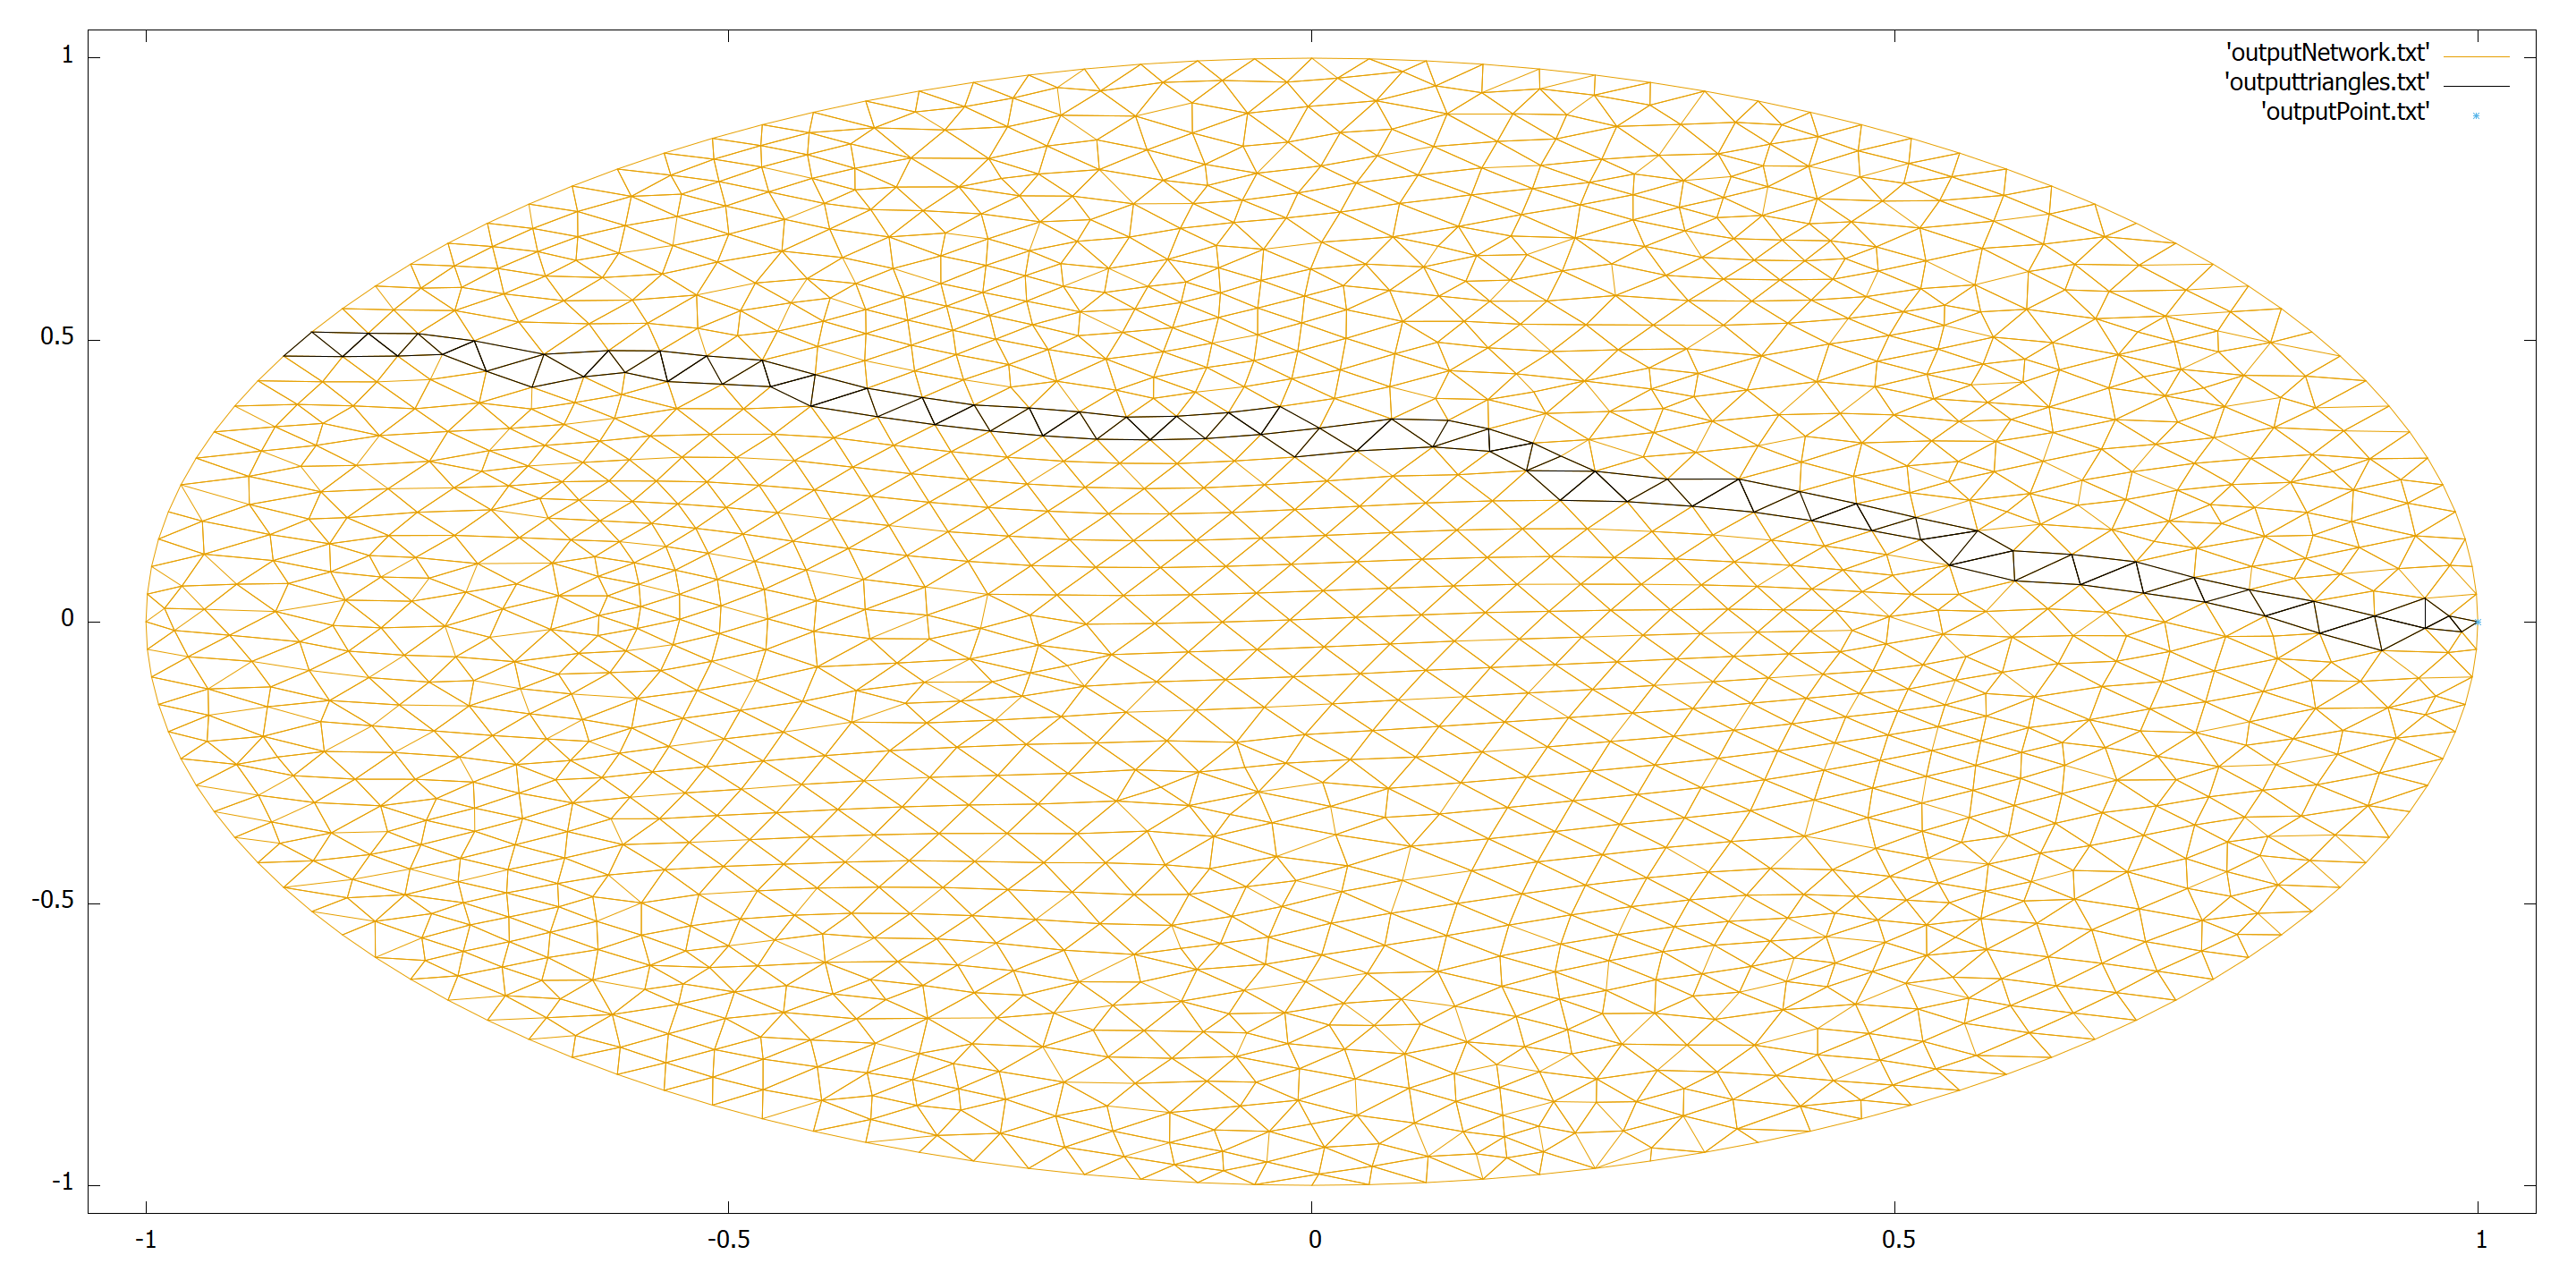
\includegraphics[width=0.55\linewidth, height=0.55\linewidth]{../Figures/StartTri600_p(1,0)_min_neg}}
%	\caption{}
	\subfigure{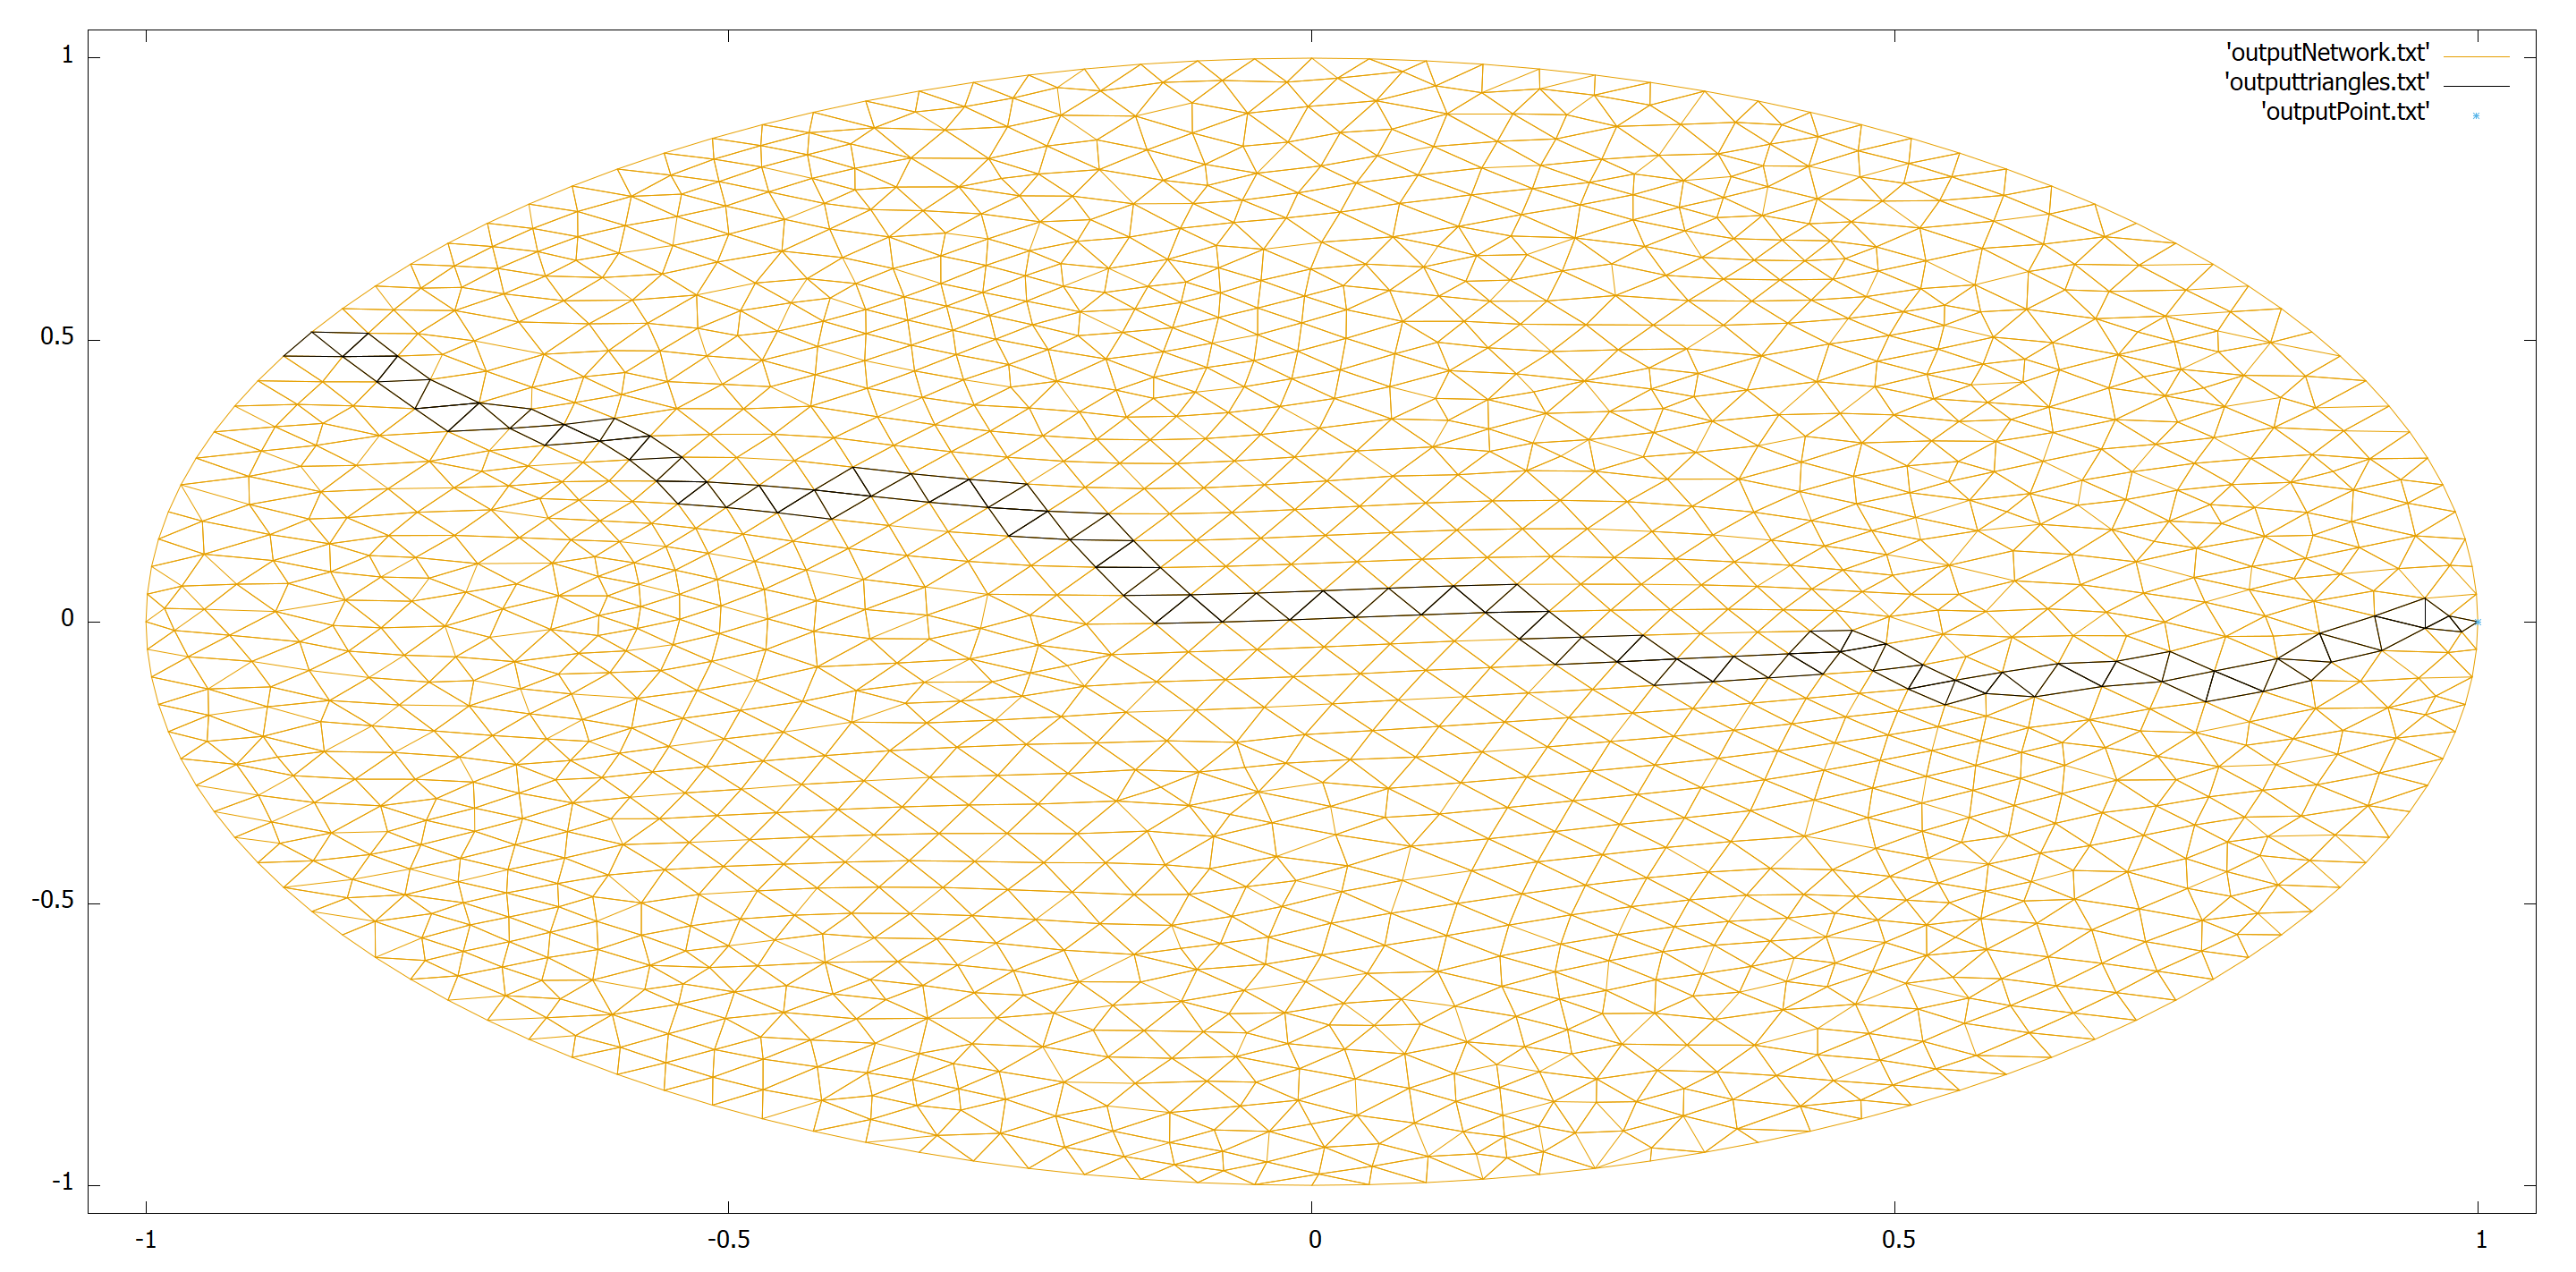
\includegraphics[width=0.55\linewidth,height=0.55\linewidth]{../Figures/StartTri600_p(1,0)_random_neg1}}
\end{figure}

\begin{figure}[h]
	\subfigure{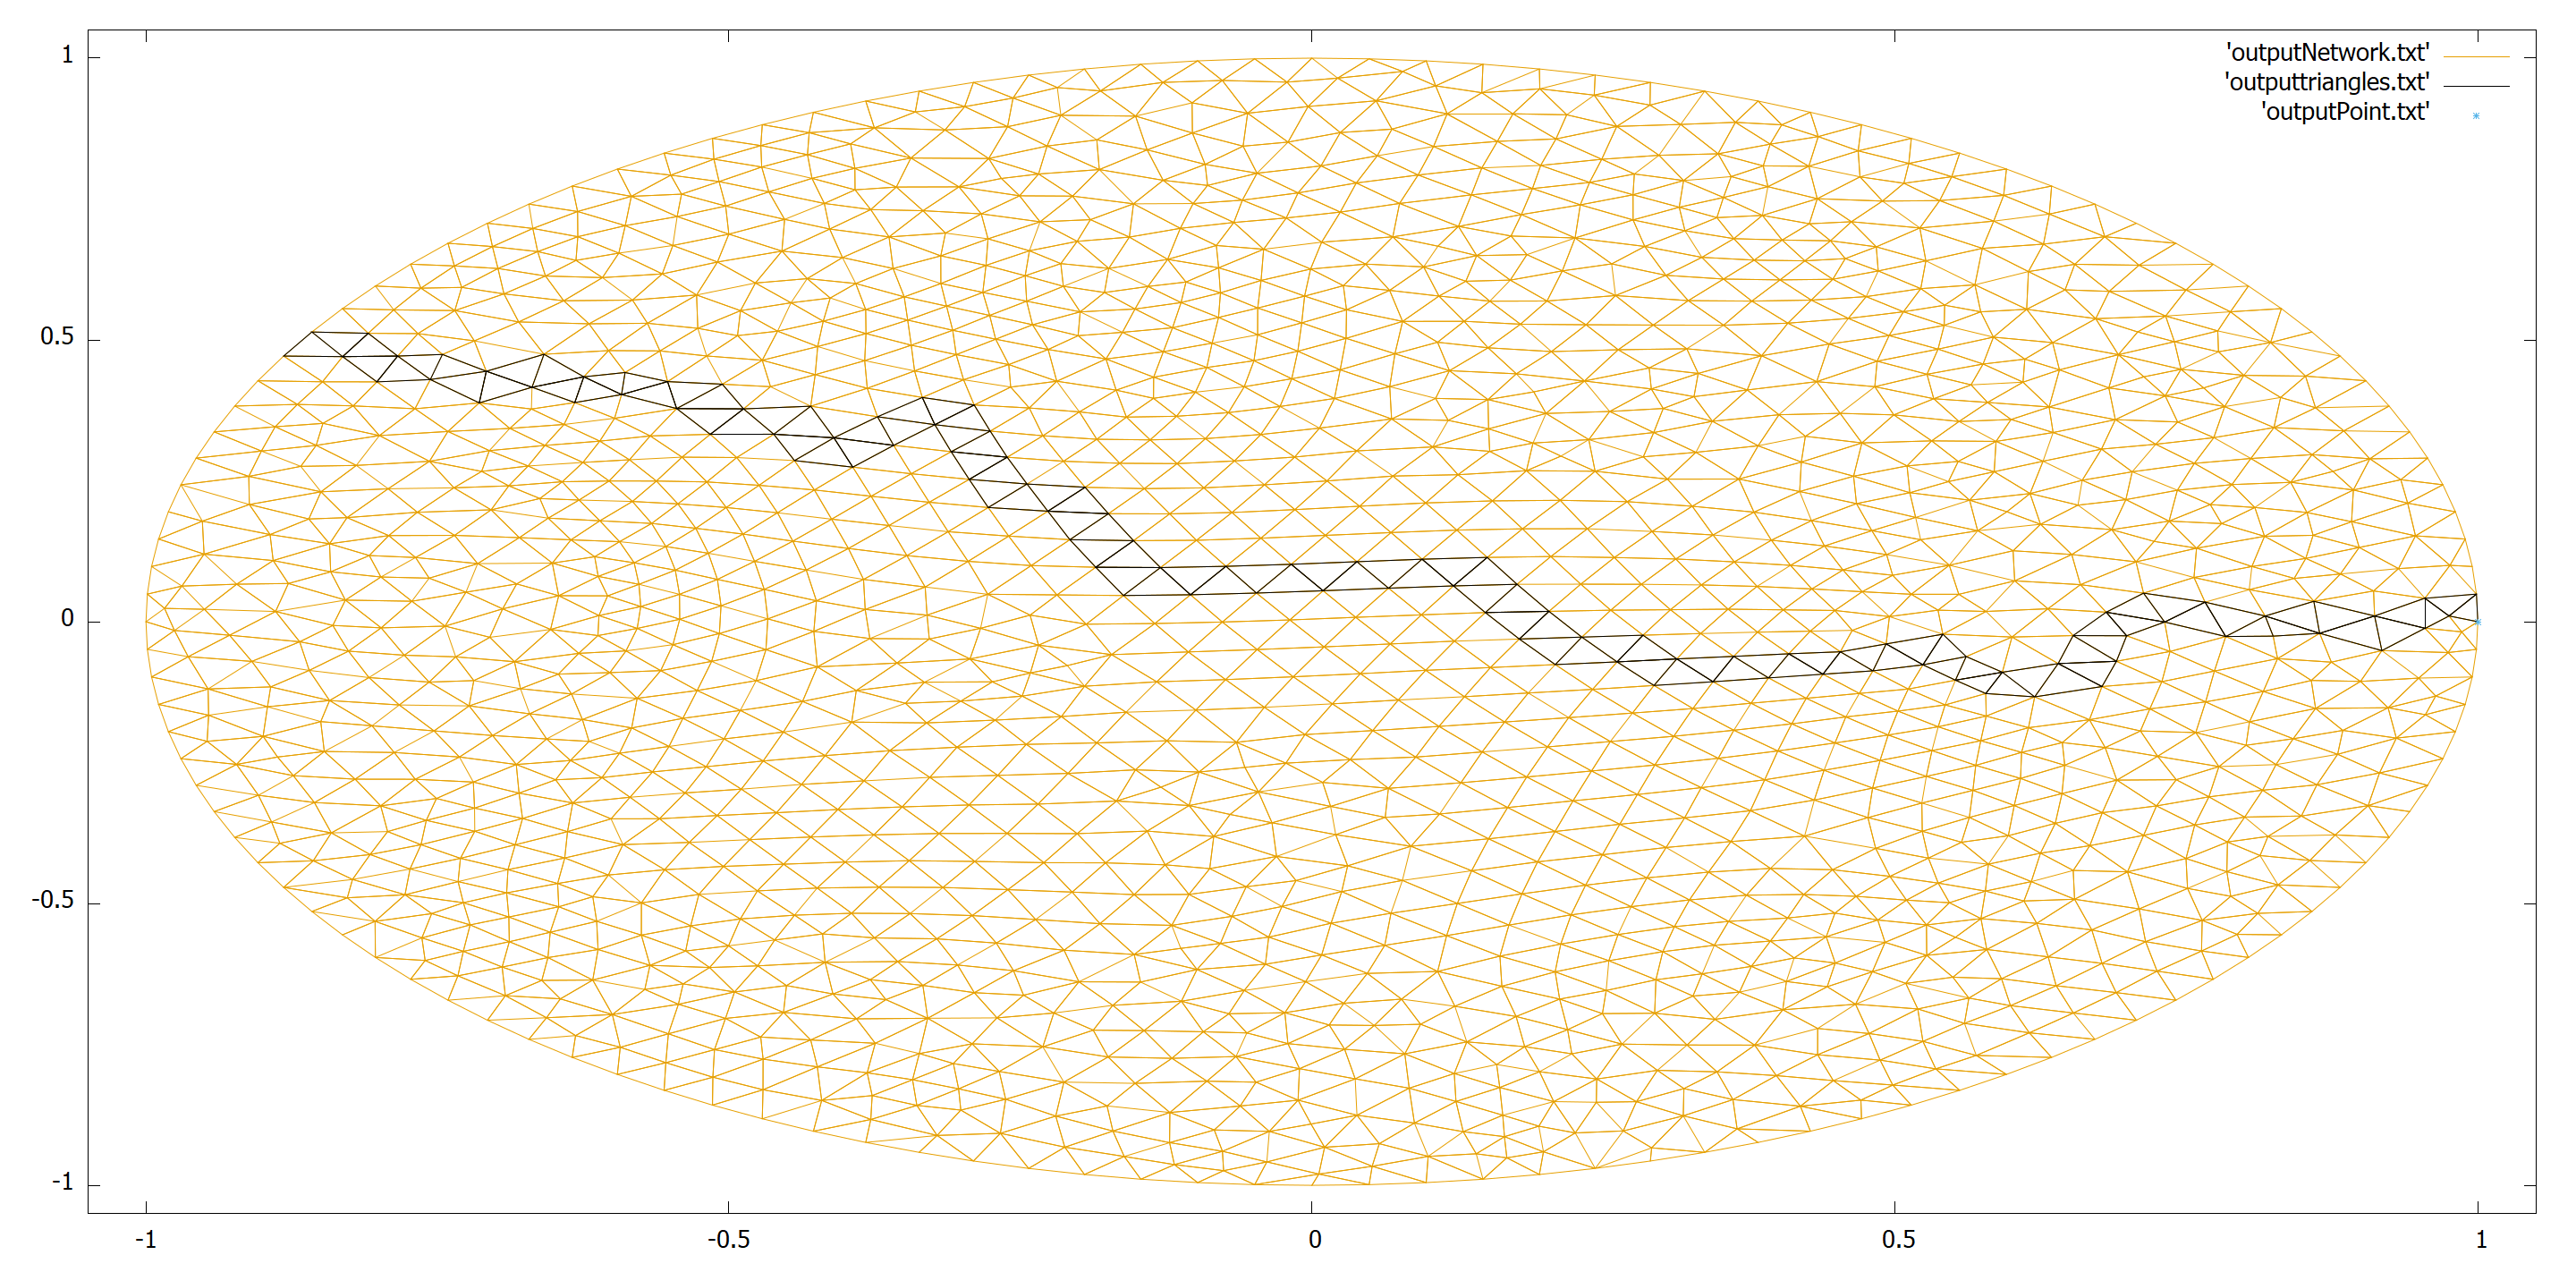
\includegraphics[width=0.55\linewidth,height=0.55\linewidth]{../Figures/StartTri600_p(1,0)_random_neg2}}
	\subfigure{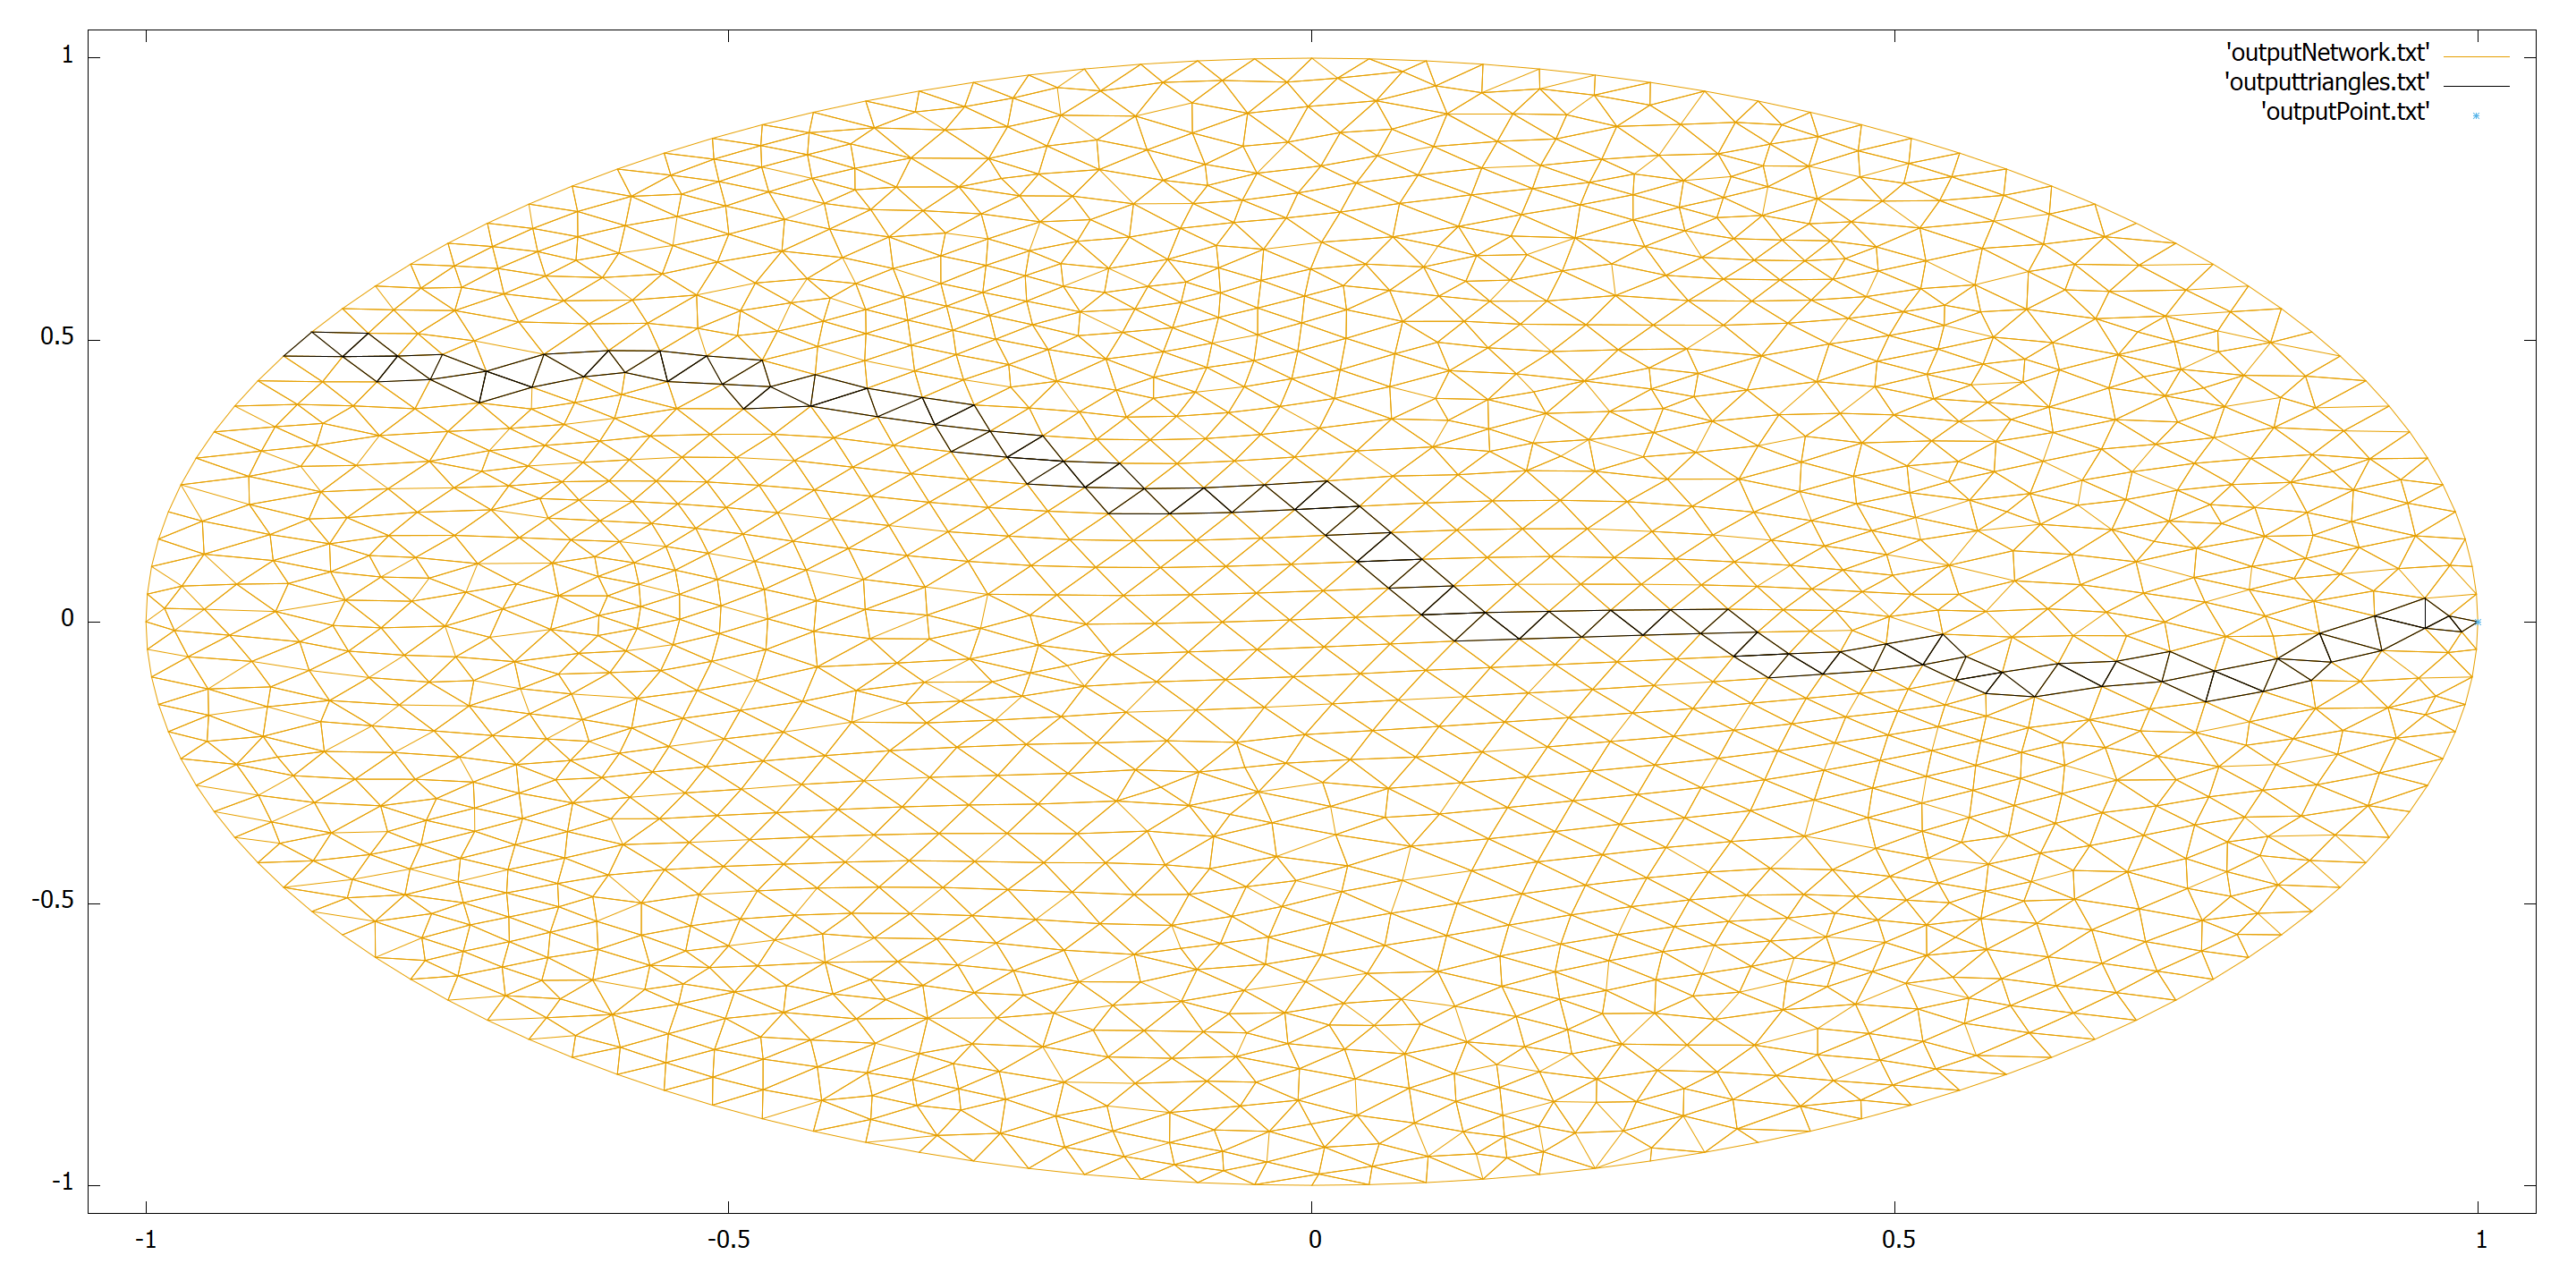
\includegraphics[width=0.55\linewidth,height=0.55\linewidth]{../Figures/StartTri600_p(1,0)_random_neg3}}
\end{figure}


\subsection{Can an arbitrary choice of the consecutive triangle be a better choice?}\label{Question}
	This example shows that a random choice of the consecutive triangle can be better. 
	\begin{figure}[h]\label{Example}
			\begin{minipage}{0.3\textwidth}
				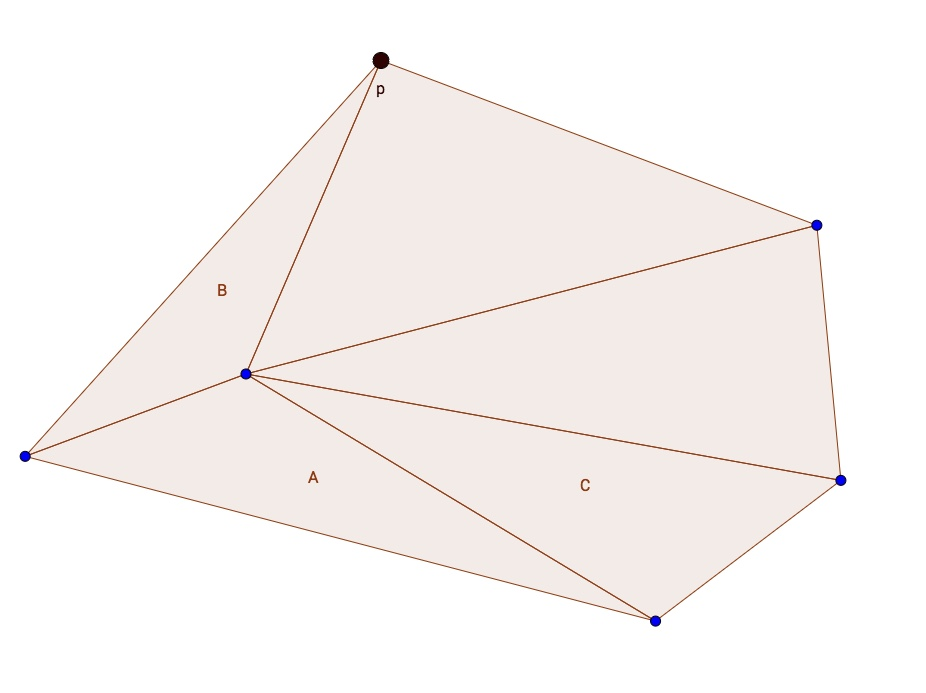
\includegraphics[scale=0.2]{../Figures/Example.jpg}
			\end{minipage}
			\hfill
			\begin{minipage}{0.4\textwidth}
				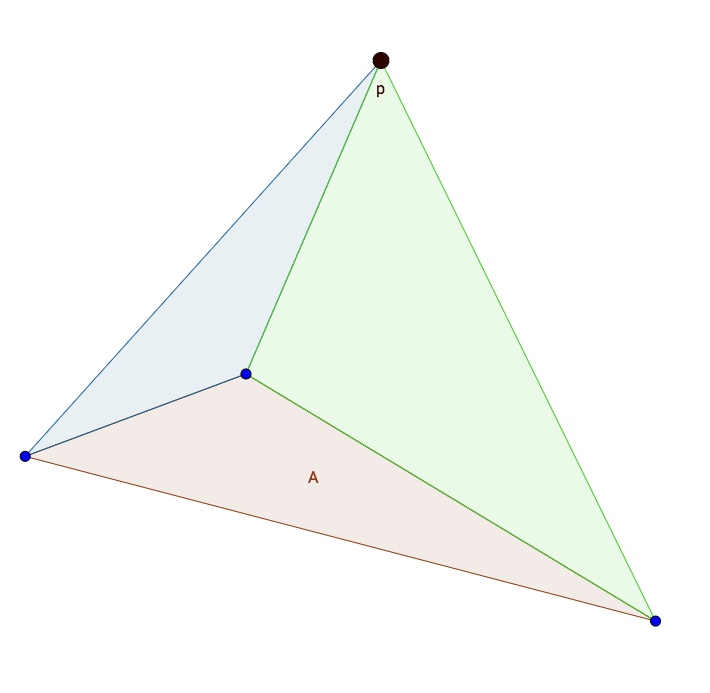
\includegraphics[scale=0.2]{../Figures/Calculation.jpg}
			\end{minipage}
		\caption{The illustration of \ref{Question}.}
			
			
	\end{figure}
	Assume that the algorithm $ promenade $ currently considers  the triangle $ A $ of figure \ref{Example} and searches for a covering triangle of the point $ p $.
	Hence, the algorithm will proceed with triangle $ B $ or $ C $. \\
	 If we use the size of the oriented volume (the oriented volume of the convex hull of $ p $ and the lower right edge of $ A $, respectively the upper right edge of $ A $) we will clearly choose $ C $, as illustrated in the second figure (the green area is clearly bigger than the blue one). This is obviously the worse choice since $ B $ is a covering triangle of the point $ p $.  \\
	 An important observation is that the regularity of the triangles plays an important role. In this case, regularity means that all triangles of the mesh have a 'similar' area, 'similar' angles and its vertices are adjacent to a 'similar' number of triangles.

\subsection{Empirical demonstration that the deterministic choice of the consecutive triangle is better in regular meshs}
If we take a look at figures \ref{30} and \ref{2000} it becomes empirically clear that the minimum choice of the consecutive triangle speeds up the algorithm. Figure \ref{30} even states that the path created by the minimum choice is always shorter or as long as the path created by the random choice. Looking at the runtime in \ref{2000} we see that the runtime is about as twice as high for the random choice when the starting triangle and the given point have a bog distance. 
 \\
Nevertheless, it has to be kept in mind that the underlying mesh plays an important role.
In this case the mesh 'maillage5.msh' is regular in the sense explained in the previous section.  

\begin{figure}[h] \label{30}
	\subfigure{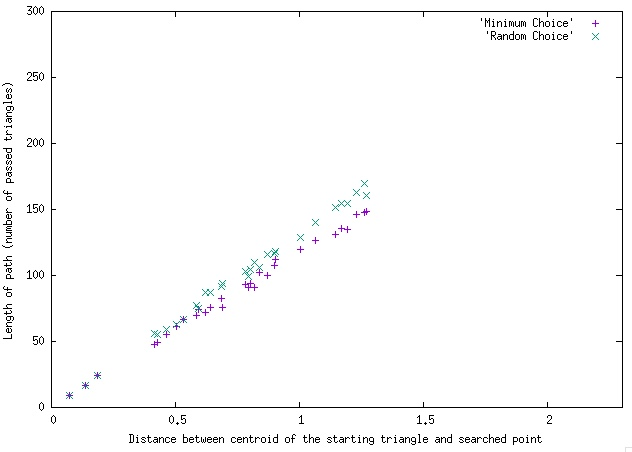
\includegraphics[width=0.5\linewidth, height=0.5\linewidth]{../Figures/Pathlength30.jpg}}
	\subfigure{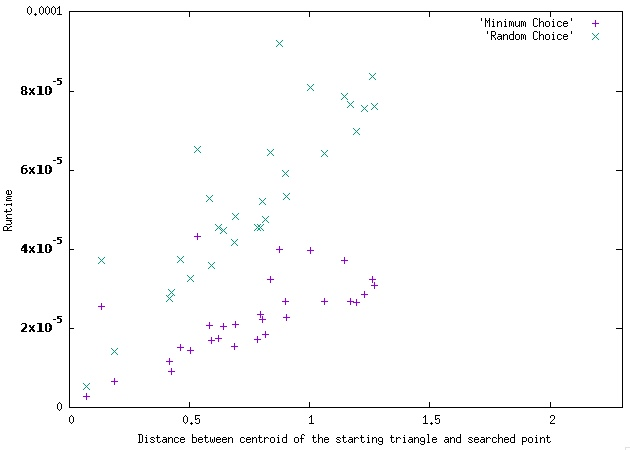
\includegraphics[width=0.5\linewidth,height=0.5\linewidth]{../Figures/Runtime30.jpg}}
	\caption{The pathlength and the runtime compared using $ min_neg $ and $ random_neg $. In this example, $ 30 $ data points were randomly created in the file 'TimeMeasurements.cpp'.  The underlying mesh is 'maillage5.msh'.}
\end{figure}

\begin{figure}[h] \label{2000}
	\subfigure{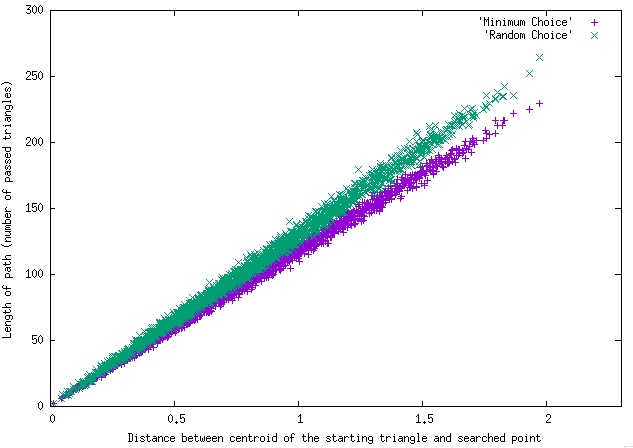
\includegraphics[width=0.5\linewidth, height=0.5\linewidth]{../Figures/Pathlength2000.jpg}}
	\subfigure{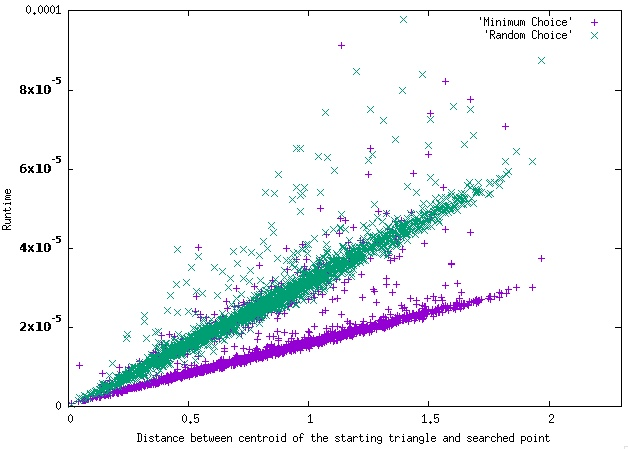
\includegraphics[width=0.5\linewidth,height=0.5\linewidth]{../Figures/Runtime2000.jpg}}
	\caption{Here, $ 2000 $ data points were randomly created.}
\end{figure}
		
		
		


\subsection{The visualization via gnuplot}
	The visualization is done by the function $ exportGnuplot $ being able to visualize two different things: 
	\begin{enumerate}
		\item 
		The result of the algorithm promenade, that is a sequence of adjacent triangles from a starting triangle to a triangle covering the searched point. 
		In this case the input variable $ triangles_path $ contains the sequence of triangles and the input variable $  points $ contains just one point, hence the input $ int numbpoints $ is $ 1 $. 
		\item 
		Given a mesh and the vertices of another mesh it can visualize the set of the covering triangles (a subset of triangles of the first mesh) of the points of the second mesh. 
		In this case the input variable $ triangles\_path $ contains the covering triangles and the $ points $ (IN VERTICES UMBENENNEN?, würde ich nicht, denn die variable heißt points und in diesem fall werden sie auch nur als points und nicht als vertices behandelt) are the vertices of the second mesh. 
	\end{enumerate}
The functions writes four text files, one for all triangles of the mesh, one for the triangles in $ triangles\_path $, one for the points in $ points $ and one for the commands which shall be executed by gnuplot. This is all realized by a simple $ ofstream $ variable, allowing to create and manipulate a text file. \\
The script for gnuplot contains a line which keeps the plot open until some key is hit in the terminal. 
The actual execution in the terminal is achieved by the command $ system $ which executes its input string in the terminal. 

\section{5 find covering Triangles}

\section{Test environment- the main function}
	The cpp file main offers the possibility to test the properties of the program:
	\begin{enumerate}
		\item 
		Find the neighbors of a triangle.
		\item 
		Find the triangle for a point (the point can be chosen).
		\item 
		Find the covering triangles for the vertices of another mesh. 
	\end{enumerate}
	All three options contain the option to choose the mesh where the mesh becomes finer from maillage1.msh increasingly to maillage5.msh. 
	Of course it is also possible to add own meshs. In this case yet, it has to be noted that the triangle's indices ordering must be increasing, as mentioned in the sections before. Moreover, the shown intervall is set 
	
\end{document}





